\subsection{IDA PRO Free}
IDA PRO Free is a disassebmler and debugging tool for binary programms.\\
It produces assembler code and controll-flow-graphs of given binarys.\\
Additionally it can extract strings and calls to system functions or external libaries as well as programm entry points. \\
It is very well documented and intuitive to use. \\
We used this tool to disassemble the binary file \code{exec} we obtained from Internet Banking. \\
It enabled us to examine the assembler code and functions used in the file. We coud rename certain variables to structurize and explain the code better. Additionally the possibility to add comments enabled us to add further informations to the code.\\
Using the informations gained this way we could reconsturct the C-code of the binary file.
\begin{figure}[ht]
	\centering
	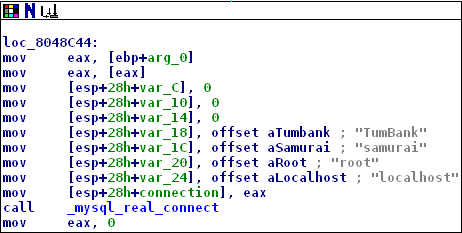
\includegraphics[width=.8\linewidth]{figures/ida_db_info.png}
	\caption{IDA PRO Free: Extracted Secrets}
	\label{fig:ida_db_info}
\end{figure}
\begin{figure}[ht]
	\centering
	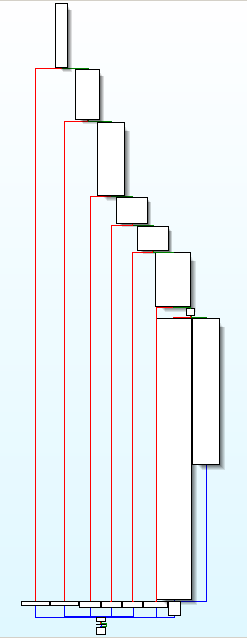
\includegraphics[width=.3\linewidth]{figures/ida_cfg_mysql_query_function.png}
	\caption{IDA PRO Free: Controll flow graph of a function}
	\label{fig:ida_controll_flow}
\end{figure}
